%======================================================================
\NEWMOD
%======================================================================

\section{\sStarting}

%----------------------------------------------------------------------

\logo{\hfill\hyperlink{outline<1>}{\icon}}

\begin{frame}[fragile,label=s-starting] 
\modframetitle{\sStarting}
\small
\begin{center}
\begin{minipage}{3.25in}
\begin{enumerate}
\item \hyperlink{ss-starting<1>}      {\BUTTON {\ssStarting}}
\item \hyperlink{ss-install-charm<1>} {\BUTTON {\ssInstallCharm}}
\item \hyperlink{ss-install-enzop<1>} {\BUTTON {\ssInstallEnzop}}
\item \hyperlink{ss-configure<1>}     {\BUTTON {\ssConfigure}}
\item \hyperlink{ss-compile<1>}       {\BUTTON {\ssCompile}}
\item \hyperlink{ss-running<1>}       {\BUTTON {\ssRunning}}
%\item \hyperlink{ss-doublemach<1>}    {\BUTTON {\ssDoubleMach}}
\item \hyperlink{ss-restart<1>}       {\BUTTON {\ssRestart}}
\item \hyperlink{ss-load-balance<1>}  {\BUTTON {\ssLoadBalance}}
\item \hyperlink{ss-tools<1>}         {\BUTTON {\ssTools}}
\item \hyperlink{ss-starting-summary<1>} {\BUTTON {\ssStartingSummary}}
\end{enumerate}
\end{minipage}
\end{center}
\end{frame}

\logo{\hfill\hyperlink{s-starting<1>}{\icon}}

%======================================================================
\NEWSEC
%======================================================================

\subsection{\ssStarting}

\begin{frame}[fragile,label=ss-starting] 
\secframetitle{\ssStarting}

Enzo-P requires several steps to download and compile

\begin{enumerate}
\item \bluetext{download and install Charm++}
\item \bluetext{download and install dependent libraries} (\redcode{hdf5, libpng} (\redcode{csh},\redcode{bc}))
\item \bluetext{download Enzo-P / Cello}
\item \bluetext{configure and compile \code{bin/enzo-p}}
\item \bluetext{run a test problem}
\end{enumerate}

\pause
\ \\
\ \\
\centerline{\redbf{Let's install and run Enzo-P!}}

\end{frame}

 % Geting started using Enzo-P / Cello
%======================================================================
\NEWSEC
%======================================================================

\subsection{\ssInstallCharm}


\begin{frame}[fragile,label=ss-install-charm] 
\secframetitle{\ssInstallCharm}
\framesubtitle{Charm++ website: \urltext{http://charm.cs.illinois.edu}}
You will likely have to download and install Charm++ yourself
\begin{center}
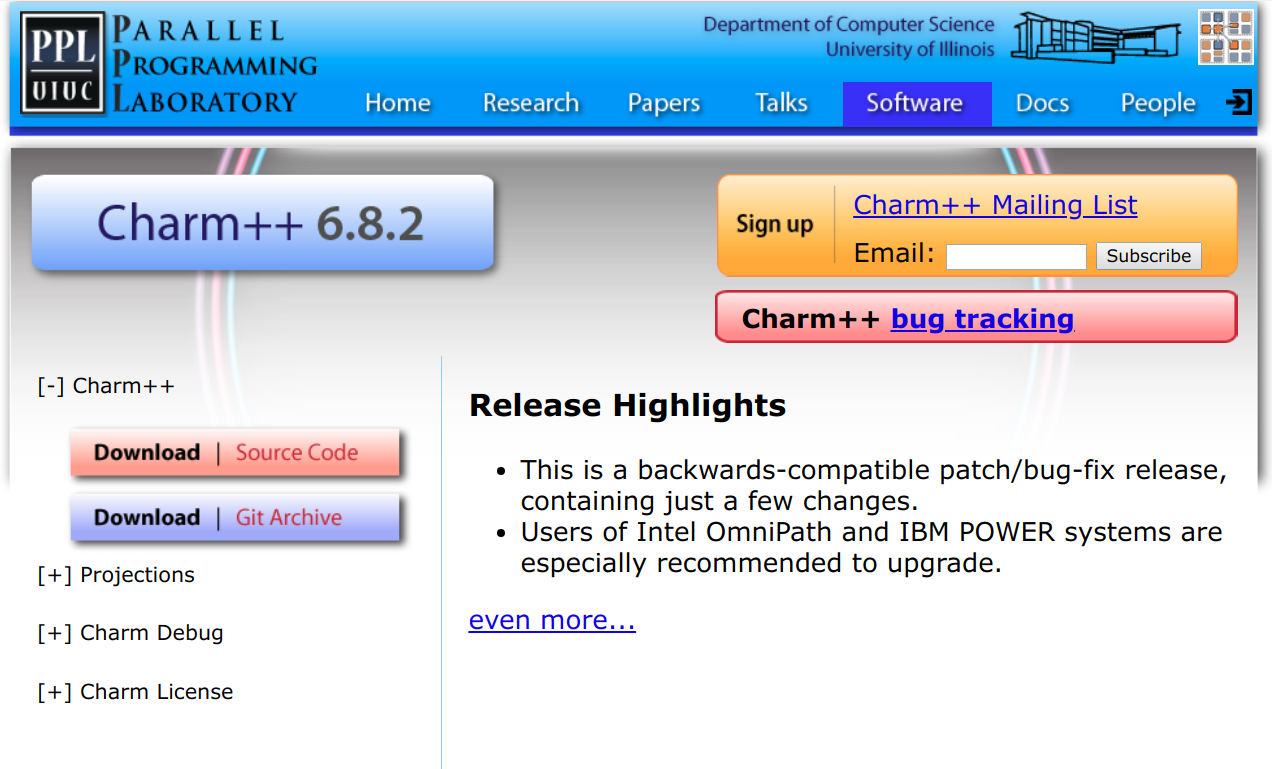
\includegraphics[width=4.00in]{charm-download.png}
\end{center}
\end{frame}


\setbeamercolor{block title}{bg=blue!30,fg=black}

%\usebackgroundtemplate
%{\includegraphics[width=5in]{monitor-2.png}}

\setbeamercolor{monitor-2.png}{bg=RGB{43,43,51}}

%----------------------------------------------------------------------

\begin{frame}[fragile] 
\secframetitle{\ssInstallCharm}
\color{black}
\footnotesize
%\begin{center}
%\begin{minipage}{3.3in}
%\begin{block}<+->{\textbf{Install \charm}}
\prompt             \redcode{ mkdir \url{~}/Charm}\cursor{1}  \\
\uncover<2->{\prompt\redcode{ cd \url{~}/Charm}\cursor{2}}  \\
\uncover<3->{\prompt\redcode{ wget http://charm.cs.illinois.edu/distrib/charm-6.8.2.tar.gz}\cursor{3}}  \\
\uncover<3->{\prompt\redcode{ (wget http://client64-249.sdsc.edu/\url{~}bordner/charm-6.8.2.tar.gz}\cursor{3})}  \\
\uncover<4->{\prompt\redcode{ tar zxf charm-6.8.2.tar.gz}\cursor{4}}  \\
\uncover<5->{\prompt\redcode{ ln -s charm-6.8.2 charm}\cursor{5}}  \\
\uncover<6->{\prompt\redcode{ cd charm}\cursor{6}}  \\
\uncover<7->{\blueit{   \#  build directly (recommended for Mac's)}} \\
\uncover<7->{\prompt\redcode{ ./build charm++ netlrts-darwin-x86\_64 gcc gfortran -j4 \textendash\textendash with-production}\cursor{7}} \\
\uncover<8->{\blueit{   \# \redbf{\textbf{or}} build directly (recommended for Linux)}} \\
\uncover<8->{\prompt\redcode{ ./build charm++ netlrts-linux-x86\_64   -j4  \textendash\textendash with-production}\cursor{8}} \\
\uncover<9->{\blueit{   \# \redbf{\textbf{or}} run the interactive build script:}} \\
\uncover<9->{\prompt\redcode{ ./smart-build.pl}\cursor{9}} \\
%\end{block}
%\end{minipage}
%\end{center}
\end{frame}


%----------------------------------------------------------------------

\begin{frame}[fragile] 
\secframetitle{\ssInstallCharm}
\framesubtitle{Compiling \charm\ with \code{./smart-build.pl}}
\color{black}
\footnotesize

\prompt\redcode{./smart-build.pl}\cursor{1}
\pause

\verb@============================================================@ \\
\ \\
\verb@Begin interactive charm configuration ...@\\
\verb@If you are a poweruser expecting a list of options, please use@ \\
\verb@   ./build --help@\\
\ \\
\verb@============================================================@ \\
\ \\
\verb@Are you building to run just on the local machine, and not across@ \\
\verb@multiple nodes? [y/N]@\cursor{2} \\
\pause
\verb@I found that you have an mpicc available in your path.@ \\
\verb@Do you want to build Charm++ on this MPI? [y/N]:@\cursor{3} \\
\end{frame}

%----------------------------------------------------------------------

\begin{frame}[fragile] 
\secframetitle{\ssInstallCharm}
\framesubtitle{Compiling \charm\ with \code{./smart-build.pl}}
\color{black}
\footnotesize

\verb@Do you have a special network interconnect? [y/N]:@\cursor{1}
\pause
\verb@y@ \\
\verb@	Choose an interconnect from below: [1-10]@ \\
\verb@		 1) MPI@ \\
\verb@		 2) Infiniband (ibverbs)@ \\
\verb@		 3) Cray XE, XK@ \\
\verb@		 4) Cray XC@ \\
\verb@		 5) Blue Gene/Q@ \\
\verb@		 6) Intel Omni-Path (ofi)@ \\
\verb@  @\cursor{2}
\end{frame}

%----------------------------------------------------------------------

\begin{frame}[fragile] 
\secframetitle{\ssInstallCharm}
\framesubtitle{Compiling \charm\ with \code{./smart-build.pl}}
\color{black}
\footnotesize

\verb@How do you want to handle SMP/Multicore: [1-3]@ \\
\verb@      1) single-threaded [default]@ \\
\verb@      2) SMP@ \\
\verb@      3) POSIX Shared Memory@ \\
\verb@  @\cursor{1}
\pause
\ \\
\verb@Do you want to specify a compiler? [y/N]@\cursor{2}\pause\verb@n@ \\
\ \\
\verb@Do you want to specify any Charm++ build options, such as fortran@ \\
\verb@   compilers? [y/N]@\cursor{3} \\

\end{frame}

%----------------------------------------------------------------------

\begin{frame}[fragile] 
\secframetitle{\ssInstallCharm}
\framesubtitle{Compiling \charm\ with \code{./smart-build.pl}}
\color{black}
\footnotesize

\verb@Choose a set of compiler flags [1-5]@ \\
\verb@	1) none@ \\
\verb@	2) debug mode                      -g -O0@ \\
\verb@	3) production build [default]      --with-production@ \\
\verb@	4) production build w/ projections --with-production --enable-tracing@ \\
\verb@	5) custom@ \\
\verb@  @\cursor{1}
\pause
\ \\ \ \\
\verb@What do you want to build?@ \\
\verb@          1) Charm++ [default] (choose this if you are building NAMD)@ \\
\verb@          2) Charm++ and AMPI@ \\
\verb@          3) Charm++, AMPI, ParFUM, FEM and other libraries@ \\
\verb@  @\cursor{2}
\end{frame}

%----------------------------------------------------------------------

\begin{frame}[fragile] 
\secframetitle{\ssInstallCharm}
\framesubtitle{Compiling \charm\ with \code{./smart-build.pl}}
\color{black}
\footnotesize
\ \\
\verb@Do you want to compile in parallel?@ \\
\verb@        1) No@ \\
\verb@        2) Build with -j2@ \\
\verb@        3) Build with -j4@ \\
\verb@        4) Build with -j8 @ \\
\verb@        5) Build with -j16 [default]@ \\
\verb@        6) Build with -j32@ \\
\verb@        7) Build with -j@ \\
\verb@  @\cursor{1}
\ \\
\pause
\verb@We have determined a suitable build line is:@ \\
\verb@	./build charm++ net-linux-x86_64  -j4  --with-production@ \\
\ \\
\verb@Do you want to start the build now? [Y/n]@\cursor{2} \pause\code{y}\\
\verb@Building with: ./build charm++ net-linux-x86_64  -j4 --with-production@

\end{frame}


%----------------------------------------------------------------------

% \begin{frame}[fragile] 
% \secframetitle{\ssInstallCharm}
% \framesubtitle{Running a \charm\ test problem}
% \color{black}
% \footnotesize
% 
% \prompt\redcode{ cd examples/charm++/hello/1darray}\cursor{1}\\\pause
% \prompt\redcode{ make test}\cursor{2}\\\pause
% 
% \color{blue}
% \verb@ ./charmrun +p4 hello 10@ \\
% \color{black}
% \verb@	Charmrun> started all node programs in 1.296 seconds. @ \\
% \verb@	Converse/Charm++ Commit ID:  @ \\
% \verb@	Trace: traceroot: /home/bordner/Charm/682/gnu/net/charm-6.8.2/examples/charm++/hello/1darray/hello @ \\
% \verb@	Charm++> scheduler running in netpoll mode. @ \\
% \verb@	CharmLB> Load balancer assumes all CPUs are same. @ \\
% \verb@	Charm++> Running on 1 unique compute nodes (8-way SMP). @ \\
% \verb@	Charm++> cpu topology info is gathered in 0.001 seconds. @ \\
% \verb@	Running Hello on 4 processors for 10 elements @ \\
% \verb@	Hello 0 created @ \\
% \verb@	Hello 1 created @ \\
% \verb@	Hello 2 created @ \\
% \verb@	Hi[17] from element 0 @ \\
% \verb@	Hi[18] from element 1 @ \\
% \verb@	Hi[19] from element 2 @ \\
% \verb@	Hello 6 created @ \ldots
% \end{frame}

\usebackgroundtemplate
{}

 % How do I download and install Charm++?
%======================================================================
\NEWSEC
%======================================================================

\subsection{\ssInstallEnzop}

%----------------------------------------------------------------------
\begin{frame}[fragile,label=ss-install-enzop] 
\secframetitle{\ssInstallEnzop}
\framesubtitle{Enzo-P source code: \url{https://bitbucket.org/cello-project}}
\footnotesize \enzopcello\ source is available from \textcolor{green!50!black}{\url{https://bitbucket.org/cello-project}}
\begin{center}
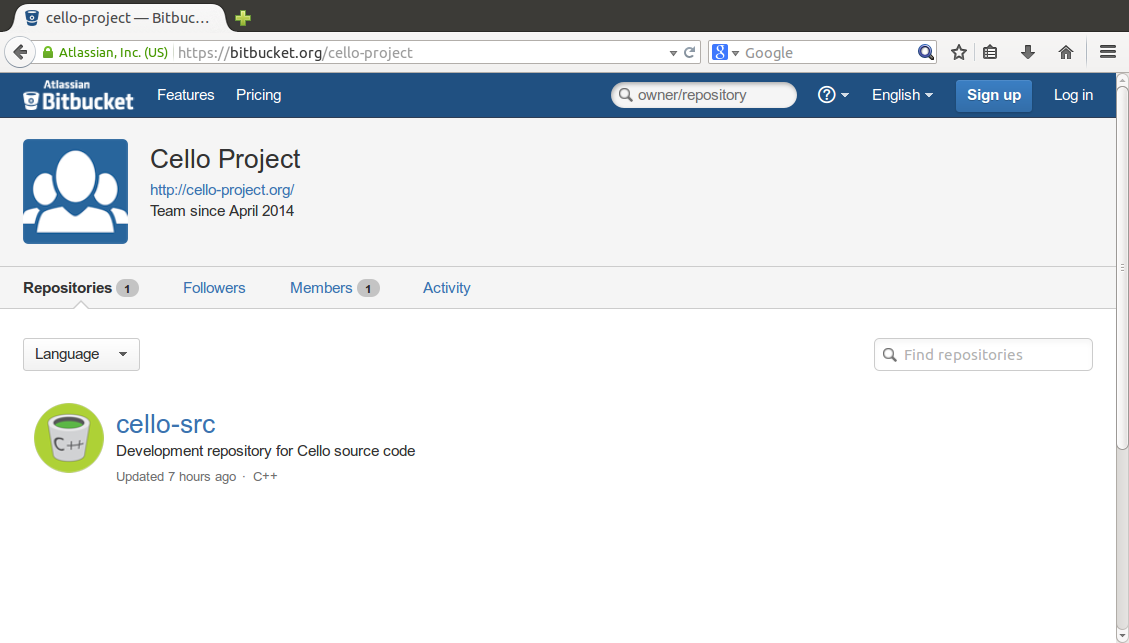
\includegraphics[width=4.00in]{cello-download.png}
\end{center}
\end{frame}
\setbeamercolor{monitor-2.png}{bg=RGB{43,43,51}}

%----------------------------------------------------------------------
\begin{frame}[fragile] 
\secframetitle{\ssInstallEnzop}
\framesubtitle{Downloading Enzo-P/Cello}
\footnotesize
\begin{semiverbatim}
 \prompt\ \redcode{hg clone https://bitbucket.org/cello-project/cello-src}\cursor{1}  
 \uncover<2->{destination directory: cello-src}
 \uncover<2->{requesting all changes}
 \uncover<2->{adding changesets} 
 \uncover<2->{adding manifests} 
 \uncover<2->{adding file changes} 
 \uncover<2->{added 3529 changesets with 21657 changes to 4353 files (+1 heads)} 
 \uncover<2->{updating to branch default} 
 \uncover<2->{resolving manifests} 
 \uncover<2->{\vdots}
 \uncover<2->{getting scons-LICENSE}
 \uncover<2->{getting scons-README}
 \uncover<2->{getting scons-local-2.2.0/SCons/Action.py}
 \uncover<2->{924 files updated, 0 files merged, 0 files removed, 0 files unresolved}
\end{semiverbatim}
\end{frame}

 % How do I download and install Enzo-P?
%======================================================================
\NEWSEC
%======================================================================

\subsection{\ssConfigure}


%    SConstruct
%    config/linux_blah

%    CELLO_PREC
%    CELLO_ARCH
%    (move prec to config?)
%   use online user documentation
%----------------------------------------------------------------------

\begin{frame}[fragile,label=ss-configure] 
\secframetitle{\ssConfigure}
%\framesubtitle{Configuring Enzo-P/Cello: \code{config/*.py}}
\footnotesize
\begin{enumerate}
\item Use or create a small config/*.py machine file
\item Set CELLO environment variables
\item Edit SConstruct user-configuration section (optional)
\end{enumerate}
\begin{semiverbatim}
 \uncover<1->{\prompt \redcode{cd cello-src}}\cursor{1}  
 \uncover<2->{\prompt \redcode{ls config}}\cursor{2} 
 \uncover<3->{\greencode{davros_gnu_debug.py   gordon_gnu.py    linux_gprof.py   ncsa_bw.py}}
 \uncover<3->{\greencode{davros_gnu.py         gordon_intel.py  linux_mpe.py}}
 \uncover<3->{\greencode{faraday_gnu_debug.py  gordon_pgi.py    mf_gnu_debug.py}}
 \uncover<3->{\greencode{faraday_gnu.py        linux_gnu.py     mf_gnu.py}}
 \uncover<4->{\prompt \redcode{export CELLO_ARCH=linux_gnu}}\cursor{4}  
 \uncover<5->{\prompt \redcode{export CELLO_PREC=single}}\cursor{5}  
 \uncover<6->{\prompt \redcode{cat config/linux_gnu.py}}\cursor{6}  
\end{semiverbatim}
\end{frame}

%----------------------------------------------------------------------
\begin{frame}[fragile] 
\secframetitle{\ssConfigure}
\framesubtitle{Configuring Enzo-P/Cello: \code{config/*.py}}
\tiny
\begin{semiverbatim}
 \uncover<1->{\prompt \redcode{cat config/linux_gnu.py}}\cursor{1}  
 \uncover<2->{import os}
 \uncover<2->{}
 \uncover<2->{is_arch_valid = 1}
 \uncover<2->{}
 \uncover<2->{flags_arch = '-Wall -O3 -g'}
 \uncover<2->{flags_link_charm = ' -rdynamic' # required for backtraces}
 \uncover<2->{}
 \uncover<2->{cc  = 'gcc '}
 \uncover<2->{f90 = 'gfortran'}
 \uncover<2->{}
 \uncover<2->{flags_prec_single = ''}
 \uncover<2->{flags_prec_double = '-fdefault-real-8 -fdefault-double-8'}
 \uncover<2->{}
 \uncover<2->{libpath_fortran = '.'}
 \uncover<2->{libs_fortran    = ['gfortran']}
 \uncover<2->{}
 \uncover<2->{use_papi=1}
 \uncover<2->{papi_inc = '/usr/local/include'}
 \uncover<2->{papi_lib = '/usr/local/lib'}
 \uncover<2->{hdf5_inc     = '/usr/include'}
 \uncover<2->{hdf5_lib     = '/usr/lib'}
 \uncover<2->{png_path     = '/lib/x86_64-linux-gnu'}
 \uncover<2->{}
 \uncover<2->{home = os.environ['HOME']}
 \uncover<2->{charm_path   = home + '/Charm/charm'}
 \uncover<2->{grackle_path = home + '/Software/Grackle/src/clib'}
\end{semiverbatim}
\end{frame}

%----------------------------------------------------------------------
\begin{frame}[fragile] 
\secframetitle{\ssConfigure}
\framesubtitle{Configuring Enzo-P/Cello: \code{SConstruct}}
\tiny
\begin{semiverbatim}
\uncover<1->{\prompt \redcode{gedit SConstruct}}\cursor{1}  

#======================================================================
# USER CONFIGURATION
#======================================================================

#----------------------------------------------------------------------
# Whether to print out detailed messages with the TRACE() series of statements
#----------------------------------------------------------------------

trace = 0

#----------------------------------------------------------------------
# Whether to trace main phases
#----------------------------------------------------------------------

verbose = 0

#----------------------------------------------------------------------
# Whether to print out messages with the TRACE_CHARM() and TRACEPUP()
#  series of statements
#----------------------------------------------------------------------

trace_charm = 0

\end{semiverbatim}
\end{frame}

%----------------------------------------------------------------------
\begin{frame}[fragile] 
\secframetitle{\ssConfigure}
\framesubtitle{Configuring Enzo-P/Cello: \code{SConstruct}}
\tiny
\begin{semiverbatim}
\uncover<1->{\prompt \redcode{gedit SConstruct}}\cursor{1}  

#----------------------------------------------------------------------
# Whether to enable displaying messages with the DEBUG() series of
# statements. Also writes messages to out.debug.<P> where P is the
# (physical) process rank. Still requires the "DEBUG" group to be
# enabled in Monitor (that is Monitor::is_active("DEBUG") must be true
# for any output)
#----------------------------------------------------------------------

debug = 0

#----------------------------------------------------------------------
# Whether to periodically print all field values.  See
# src/Field/field_FieldBlock.cpp
#----------------------------------------------------------------------

debug_verbose = 0

\end{semiverbatim}
\end{frame}

%----------------------------------------------------------------------
\begin{frame}[fragile] 
\secframetitle{\ssConfigure}
\framesubtitle{Configuring Enzo-P/Cello: \code{SConstruct}}
\tiny
\begin{semiverbatim}
\uncover<1->{\prompt \redcode{gedit SConstruct}}\cursor{1}  

#----------------------------------------------------------------------
# Whether to track dynamic memory statistics.  Can be useful, but can
# cause problems on some systems that also override new [] () / delete
# [] ()
#----------------------------------------------------------------------

memory = 1

#----------------------------------------------------------------------
# Enable charm++ dynamic load balancing
#----------------------------------------------------------------------

balance = 1

\end{semiverbatim}
\end{frame}

%----------------------------------------------------------------------
\begin{frame}[fragile] 
\secframetitle{\ssConfigure}
\framesubtitle{Configuring Enzo-P/Cello: \code{SConstruct}}
\tiny
\begin{semiverbatim}
\uncover<1->{\prompt \redcode{gedit SConstruct}}\cursor{1}  
#----------------------------------------------------------------------
# Whether to compile with -pg to use gprof for performance profiling
#----------------------------------------------------------------------

use_gprof = 0

#----------------------------------------------------------------------
# Whether to compile with the Grackle chemistry and cooling library
#
# WARNING: must update grackle-related lines in src/Enzo/enzo.ci
#----------------------------------------------------------------------

use_grackle = 0

#----------------------------------------------------------------------
# Whether to run the test programs using valgrind to check for memory leaks
#----------------------------------------------------------------------

use_valgrind = 0

\end{semiverbatim}
\end{frame}

%----------------------------------------------------------------------
\begin{frame}[fragile] 
\secframetitle{\ssConfigure}
\framesubtitle{Configuring Enzo-P/Cello: \code{SConstruct}}
\tiny
\begin{semiverbatim}
\uncover<1->{\prompt \redcode{gedit SConstruct}}\cursor{1}  
#----------------------------------------------------------------------
# Whether to use Cello Performance class for collecting performance
# data (currently requires global reductions, and may not be fully
# functional) (basic time data on root processor is still output)
#----------------------------------------------------------------------

use_performance = 0

#----------------------------------------------------------------------
# Whether to compile the CHARM++ version for use with the Projections
# performance tool.
#----------------------------------------------------------------------

use_projections = 0

#----------------------------------------------------------------------
# How many processors to run parallel unit tests
#----------------------------------------------------------------------

ip_charm = '4'

#----------------------------------------------------------------------
# Whether this is a Mercurial repository
#----------------------------------------------------------------------

have_mercurial = 1
\end{semiverbatim}
\end{frame}

 % How do I configure Enzo-P?
%======================================================================
\NEWSEC
%======================================================================

\subsection{\ssCompile}

%----------------------------------------------------------------------
\begin{frame}[fragile,label=ss-compile] 
\secframetitle{\ssCompile}
\framesubtitle{Compiling Enzo-P/Cello}
\tiny
\begin{semiverbatim}
\uncover<1->{\prompt \redcode{make}}\cursor{1}  
\uncover<2->{./build.sh bin/enzo-p
Remove bin/enzo-p
2015-09-19 14:36:00 BEGIN
BEGIN Enzo-P/Cello ./build.sh
arch = linux_gnu
prec = double
target = bin/enzo-p
2015-09-19 14:36:00 compiling...                 PAPI installed

    CELLO_ARCH scons arch= linux_gnu
    CELLO_PREC scons prec= double

scons: warning: Two different environments were specified for target main_enzo.o,
	but they appear to have the same action: $CXX -o $TARGET -c $CXXFLAGS $CCFLAGS $_CCCOMCOM $SOURCES
File "/home/bordner/Cello/cello-src/build/Cello/SConscript", line 197, in <module>
/home/bordner/Charm/charm/bin/charmc -language charm++ -o build/Enzo/enzo-p.o -c -Wall -O3 -g -balancer Greed}
\uncover<3->{\vdots}
\uncover<4->{Install file: "build/Enzo/enzo-p" as "bin/enzo-p"
Success
done
END   Enzo-P/Cello ./build.sh: arch = linux_gnu  prec = double  target = bin/enzo-p time = 77s}
\uncover<5->{\prompt \redcode{charmrun +p4 bin/enzo-p input/test_implosion.in}}\cursor{5}
\end{semiverbatim}
\end{frame}

%----------------------------------------------------------------------
%\begin{frame}[fragile] 
% \secframetitle{\ssCompile}
%\framesubtitle{\url{https://bitbucket.org/cello-project/cello-src}}
%\footnotesize
%\begin{semiverbatim}
%% \uncover<1->{\prompt charmrun +p4 bin/enzo-p input/test_implosion.in}\cursor{9}

%\end{semiverbatim}
%\end{frame}

%   use online user documentation
%    generates
%       ./bin/enzo-p
%       ./errors.org

 % How do I compile Enzo-P?
%======================================================================
\NEWSEC
%======================================================================

\subsection{\ssRunning}

\begin{frame}[fragile,label=ss-running] 
\secframetitle{\ssRunning}
\framesubtitle{Enzo-P output: header text}
\tiny
\begin{semiverbatim}
\uncover<1->{\prompt \redcode{charmrun +p4 bin/enzo-p input/test_implosion.in}}\cursor{1}
\uncover<2->{Charmrun> started all node programs in 1.298 seconds.
Converse/Charm++ Commit ID: 
Charm++> scheduler running in netpoll mode.
CharmLB> Load balancer assumes all CPUs are same.
Charm++> Running on 1 unique compute nodes (8-way SMP).
Charm++> cpu topology info is gathered in 0.002 seconds.
UNIT TEST BEGIN
0 00001.06  ==============================================
0 00001.06  
0 00001.06    .oooooo.             oooo  oooo            
0 00001.06   d8P'  `Y8b            `888  `888            
0 00001.06  888           .ooooo.   888   888   .ooooo.  
0 00001.06  888          d88' `88b  888   888  d88' `88b 
0 00001.06  888          888ooo888  888   888  888   888 
0 00001.06  `88b    ooo  888    .o  888   888  888   888 
0 00001.06   `Y8bood8P'  `Y8bod8P' o888o o888o `Y8bod8P' 
0 00001.06  
0 00001.06  A Parallel Adaptive Mesh Refinement Framework
0 00001.06  
0 00001.06    Laboratory for Computational Astrophysics
0 00001.06          San Diego Supercomputer Center
0 00001.06       University of California, San Diego
0 00001.06  See 'LICENSE_CELLO' for software license information}
\end{semiverbatim}
\end{frame}
\begin{frame}[fragile]
\secframetitle{\ssRunning}
\framesubtitle{Enzo-P output: configuration settings}
\tiny
\begin{semiverbatim}
0 00001.06  BEGIN CELLO: Sep 19 14:37:45
0 00001.06 Define Simulation processors 4
0 00001.06 Define CELLO_ARCH linux_gnu
0 00001.06 Define CELLO_PREC double
0 00001.06 Define CC            gcc 
0 00001.06 Define CFLAGS        -Wall -O3 -g   
0 00001.06 Define CPPDEFINES    CONFIG_PRECISION_DOUBLE SMALL_INTS H5_USE_16_API NO_FREETYPE CONFIG_USE_PAPI 
PAPI3 CONFIG_USE_MEMORY CONFIG_HAVE_MERCURIAL CONFIG_USE_CHARM CONFIG_USE_CELLO
0 00001.06 Define CPPPATH       #/include /usr/local/include /usr/include
0 00001.06 Define CXX           /home/bordner/Charm/charm/bin/charmc -language charm++  
0 00001.06 Define CXXFLAGS      -Wall -O3 -g     -balancer GreedyCommLB -balancer GreedyLB -balancer HybridLB
 -balancer NeighborLB -balancer RandCentLB -balancer RefineCommLB -balancer RefineLB -balancer RotateLB
0 00001.06 Define FORTRANFLAGS  -Wall -O3 -g    -fdefault-real-8 -fdefault-double-8
0 00001.06 Define FORTRAN       gfortran
0 00001.06 Define FORTRANLIBS   gfortran
0 00001.06 Define FORTRANPATH   #/include
0 00001.06 Define LIBPATH       #/lib /usr/local/lib /usr/lib /lib/x86_64-linux-gnu/lib .
0 00001.06 Define LINKFLAGS     -Wall -O3 -g     -module GreedyCommLB -module GreedyLB -module HybridLB -modu
le NeighborLB -module RandCentLB -module RefineCommLB -module RefineLB -module RotateLB
0 00001.06 Define BUILD HOST    gedeckt
0 00001.06 Define BUILD DIR     /home/bordner/Cello/cello-src
0 00001.06 Define BUILD DATE    2015-09-19
0 00001.06 Define BUILD TIME    21:36:02
0 00001.06 Define CHARM_VERSION 60500
0 00001.06 Define CHANGESET     3841+
\end{semiverbatim}
\end{frame}
\begin{frame}[fragile]
\secframetitle{\ssRunning}
\framesubtitle{Enzo-P output: parameters accessed}
\tiny
\begin{semiverbatim}
0 00001.06  BEGIN ENZO-P
0 00001.06 Memory bytes 1013270 bytes_high 1013301
0 00001.06 Parameters read in input/test_implosion.in
0 00001.06 Parameters accessed Adapt:interval 1 [default]
0 00001.06 Parameters accessed Adapt:list[0] "SLOPE"
0 00001.06 Parameters accessed Adapt:SLOPE:type "slope"
0 00001.06 Parameters accessed Adapt:min_face_rank 0 [default]
0 00001.06 Parameters accessed Adapt:SLOPE:field_list[0] "density"
0 00001.06 Parameters accessed Adapt:SLOPE:min_refine 0.30000000000000 [default]
0 00001.06 Parameters accessed Adapt:SLOPE:max_coarsen 0.15000000000000 [default]
0 00001.06 Parameters accessed Adapt:SLOPE:max_level 2147483647 [default]
0 00001.06 Parameters accessed Adapt:SLOPE:level_exponent 0.0000000000000 [default]
0 00001.06 Parameters accessed Adapt:SLOPE:output  [default]
0 00001.06 Parameters accessed Adapt:SLOPE:include_ghosts false [default]
0 00001.06 Parameters accessed Boundary:type "reflecting"
0 00001.06 Parameters accessed Boundary:axis all [default]
0 00001.06 Parameters accessed Boundary:face all [default]
0 00001.06 Parameters accessed Domain:lower[0] 0.0000000000000
0 00001.06 Parameters accessed Domain:upper[0] 0.30000000000000
\vdots
\end{semiverbatim}
\end{frame}
\begin{frame}[fragile]
\secframetitle{\ssRunning}
\framesubtitle{Enzo-P output: simulation cycles}
\tiny
\begin{semiverbatim}
0 00002.07  -------------------------------------
0 00002.07 Simulation cycle 0000
0 00002.07 Simulation time-sim 0.000000000000e+00
0 00002.07 Simulation dt 0.000000000000e+00
0 00002.07 Performance unknown time-usec 0
0 00002.07 Performance simulation time-usec 3927213
0 00002.07 Performance cycle time-usec 0
0 00002.07 Performance cycle bytes-curr 0
0 00002.07 Performance cycle bytes-high 0
0 00002.07 Performance cycle bytes-highest 0
0 00002.07 Performance initial time-usec 971452
0 00002.07 Performance adapt time-usec 1326831
0 00002.07 Performance refresh time-usec 0
0 00002.07 Performance compute time-usec 0
0 00002.07 Performance output time-usec 1608215
0 00002.07 Performance stopping time-usec 0
0 00002.07 Performance simulation num-blocks 184
0 00002.07  -------------------------------------
\end{semiverbatim}
\end{frame}

%----------------------------------------------------------------------

\begin{frame}[fragile]
\secframetitle{\ssRunning}
\begin{minipage}{2.5in}
\only<1->{\ANIMATEGRAPHICS{width=2.5in}{20}{Images/Implosion/d-}{000}{200}}
\end{minipage}
%\begin{minipage}{2in}
%\only<2->{\ANIMATEGRAPHICS{width=2.0in}{20}{Images/Implosion/implosion-mesh-}{000}{200}}
%\end{minipage}
\end{frame}

 % How do I run an example problem?
%%======================================================================
\NEWSEC
%======================================================================

\subsection{\ssDoubleMach}

\begin{frame}[fragile,label=ss-doublemach] 
\secframetitle{\ssDoubleMach}
\framesubtitle{Test problem specification}

\footnotesize
\begin{center}

\includegraphics[width=4.0in]{Images/DoubleMachAmr/doublemach-de-0000.png}
\end{center}

\begin{tabbing}
xxxxxxxxxxxxxxxxxxxxxxxxxxxxxxxx\=xxxxxxxxxxxxxxxxxxx\=\kill
\> \bluetext{Adiabatic index}: \' $\gamma = 1.4$. \\
\> \bluetext{Grid domain}: \' $0.0 < x < 4.0$, $0.0 < y < 1.0$ \\
\> \bluetext{Shock}: \' Mach 10, $v_s$ = 10.0, \\
\> \bluetext{Angle}: \' 30 degrees. \\
\> \bluetext{Pre-shock conditions}: \' $P = 1.0$, $\rho = 1.4$, $v = 0.0$ \\
\> \bluetext{Post-shock conditions}: \' $P = 116.5$, $\rho = 8$, $v = 8.25$ \\
\> \bluetext{Time limit}: \' $t = 0.25$.
\end{tabbing}
\end{frame}

%----------------------------------------------------------------------

\begin{frame}[fragile] 
\secframetitle{\ssDoubleMach}
\framesubtitle{\group{Domain} and \group{Stopping} criteria}
\begin{itemize}
\item \group{Domain}

\begin{itemize}
\item $0.0 < x < 4.0, 0.0 < y < 1.0$
\begin{semiverbatim}
\group{Domain} \{ 
   \parameter{lower} = [\valuetext{0.0}, \valuetext{0.0}];
   \parameter{upper} = [\valuetext{4.0}, \valuetext{1.0}];
\} 
\end{semiverbatim}
\end{itemize}
%
\item \group{Stopping} criteria
\begin{itemize}
%
\item $t=0.25$
%
\begin{semiverbatim}
\group{Stopping} \{ \variable{time} = \valuetext{0.25}; \} 
\end{semiverbatim}
%
\end{itemize}
\end{itemize}
\end{frame}

%----------------------------------------------------------------------

 \begin{frame}[fragile] 
 \secframetitle{\ssDoubleMach}
 \framesubtitle{\group{Initial} conditions}
\footnotesize
Complex initial conditions can be specified directly.

 \begin{itemize}
 \item To specify $x = a(x,y,z)$ in subregion $A$, else $x = b(x,y,z)$:
 \begin{tabbing}
 xxxxxxx\=\kill
\parameter{x} = \code{[} \> \valuetext{a(x,y,z)} \comment{\# (floating-point expression)}, \\
\>                         \valuetext{A(x,y,z)} \comment{\# (logical expression)}, \\
\>                         \valuetext{b(x,y,z)} \comment{\# (floating-point expression)} ];
 \end{tabbing}
 \item E.g. to specify ``$\rho = 8$ if $x \le 1/6 + 0.57735 y$, else $\rho = 1.4$'':
\begin{semiverbatim}
\group{Initial} \{
    \subgroup{density} \{
        \parameter{value} = [\valuetext{8.0}, \valuetext{(x <= 0.16667 + 0.57735*y)}, 
                 \valuetext{1.4}];  \};
\}
\end{semiverbatim}
\item Repeat with \subgroup{velocity\_x}, \subgroup{velocity\_y}, \subgroup{total\_energy}
 \end{itemize}
\end{frame}

%----------------------------------------------------------------------

\begin{frame}[fragile] 
\secframetitle{\ssDoubleMach}
\framesubtitle{\group{Initial} conditions}
\footnotesize
\begin{itemize}
\item Repeat with \subgroup{velocity\_x}, \subgroup{velocity\_y}, and \subgroup{total\_energy}
\begin{semiverbatim}
\group{Initial} \{
    \subgroup{velocity_x} \{
       \parameter{value} = [ \valuetext{8.25*0.8660253},
                        \valuetext{(x <= 0.16667 + 0.57735*y)},
                 \valuetext{0.0} ]; \};
    \subgroup{velocity_y} \{
       \parameter{value} = [\valuetext{-8.25*0.5},
                        \valuetext{(x <= 0.16667 + 0.57735*y)},
                 \valuetext{0.0}]; \};
    \subgroup{total_energy} \{
       \parameter{value} = [\valuetext{116.5 / (0.4 * 8.0) + 34.03125},
                        \valuetext{(x <= 0.16667 + 0.57735*y)}, 
                  \valuetext{1.0 / (0.4 * 1.4)}]; \};
 \}
\end{semiverbatim}
\end{itemize}
\end{frame}

%----------------------------------------------------------------------

 \begin{frame}[fragile] 
 \secframetitle{\ssDoubleMach}
 \framesubtitle{\group{Boundary} conditions}
\footnotesize
Complex boundary conditions can also be specified directly.

\begin{itemize}
\item General form:
 \begin{tabbing}
xxx\=xxx\=\kill
\group{Boundary} \{ \\
\>   \parameter{list} = [ \valuetext{"bc\_1"}, \valuetext{"bc\_2"}, \valuetext{"bc\_3"}, ... ];  \\
\\
\>   \subgroup{bc\_1} \{ \\
\>\>      \parameter{type} = \textit{\{} \valuetext{"inflow"}, \valuetext{"periodic"}, \valuetext{"outflow"}, \valuetext{"reflecting"} \textit{\}} \\
\>\>      \parameter{mask} = \valuetext{M(x,y,z,t)}; \comment{\# (logical expression)} \\
\>\>      \parameter{axis} = \textit{\{} \valuetext{"x"}, \valuetext{"y"}, \valuetext{"z"} \textit{\}} \\
\>\>      \parameter{face} = \textit{\{} \valuetext{"lower"}, \valuetext{"upper"}  \textit{\}} \\
\>\>      \parameter{field\_list} = [ \valuetext{velocity\_x} ]; \\
\>\>      \parameter{value} = \valuetext{M(x,y,z,t)}; \comment{\# (floating-point expression, inflow only)} \\
\>   \}; \\
\>   \subgroup{bc\_2} \{ \ldots \} \\
\}
\end{tabbing}
\end{itemize}
\end{frame}
%  
%  % 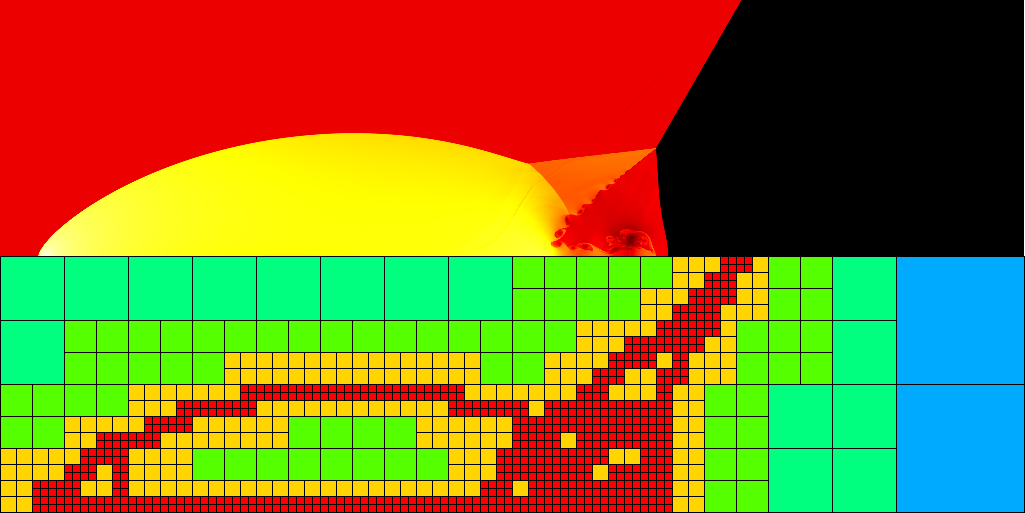
\includegraphics[width=4.0in]{Images/DoubleMachAmr/doublemach-0200.png}
%  % \ANIMATEGRAPHICS{width=4.5in}{20}{Images/DoubleMachAmr/doublemach-}{0000}{0307}
%  
%  
%  %    Boundary
%  %----------------------------------------------------------------------
%  
 \begin{frame}[fragile] 
 \secframetitle{\ssDoubleMach}
 \framesubtitle{\group{Boundary} conditions}
\footnotesize
\begin{semiverbatim}
 \group{Boundary} \{
    \variable{list} = [
            \valuetext{"OUT"},
            \valuetext{"REFLECT"},
            \valuetext{"DENSITY"},
            \valuetext{"VELOCITY_X"},
            \valuetext{"VELOCITY_Y"},
            \valuetext{"TOTAL_ENERGY}"
          ];
\}
\end{semiverbatim}
\end{frame}

%----------------------------------------------------------------------

 \begin{frame}[fragile] 
 \secframetitle{\ssDoubleMach}
 \framesubtitle{\group{Boundary} conditions: outflow and reflecting}
\footnotesize
\begin{semiverbatim}
 \group{Boundary} \{
    \subgroup{OUT} \{
       \variable{type} = \valuetext{"outflow"};
       \variable{mask} = [ (\variable{x} >= \valuetext{4.0}) || 
                (\variable{y} >= \valuetext{1.0} && (\variable{x} >= \valuetext{0.744017} + \valuetext{11.547}* \variable{t}))];
    \};
    \subgroup{REFLECT} \{
       \variable{type} = \valuetext{"reflecting"};
       \variable{axis} = \valuetext{"y"};
       \variable{face} = \valuetext{"lower"};
       \variable{mask} = (\variable{x} >= \valuetext{0.166667});
    \};
\} 
\end{semiverbatim}
\end{frame}

%----------------------------------------------------------------------

 \begin{frame}[fragile] 
 \secframetitle{\ssDoubleMach}
 \framesubtitle{\group{Boundary} conditions: \code{density}}
\footnotesize
\begin{semiverbatim}
\group{Boundary} \{
    \subgroup{DENSITY} \{
       \variable{type} = \valuetext{"inflow"};
       \variable{field_list} = \valuetext{"density"};
       \variable{value} = [ \valuetext{8.0}, 
                  ( (\variable{x} <= \valuetext{0.166667}) && (\variable{y} <= \valuetext{0.0}) ) ||
                    (\variable{x} <= \valuetext{0.0}) ||
                   ((\variable{x} <= \valuetext{0.744017} + \valuetext{11.547}*\variable{t)} && (\variable{y} >= \valuetext{1.0}))
               ];
    \};
\} 
\end{semiverbatim}
\end{frame}

%----------------------------------------------------------------------

 \begin{frame}[fragile] 
 \secframetitle{\ssDoubleMach}
 \framesubtitle{\group{Boundary} conditions: \code{velocity\_x}}
\footnotesize
\begin{semiverbatim}
\group{Boundary} \{
    \subgroup{VELOCITY_X} \{
       \variable{type} = \valuetext{"inflow"};
       \variable{field_list} = \valuetext{"velocity_x"};
       \variable{value} = [ \valuetext{8.25}*\valuetext{0.8660253},
                  ( (\variable{x} <= \valuetext{0.166667}) && (\variable{y} <= \valuetext{0.0}) ) ||
                    (\variable{x} <= \valuetext{0.0}) ||
                   ((\variable{x} <= \valuetext{0.744017} + \valuetext{11.547}*\variable{t)} && (\variable{y} >= \valuetext{1.0}))
               ];
    \};
\}
\end{semiverbatim}
\end{frame}

%----------------------------------------------------------------------

 \begin{frame}[fragile] 
 \secframetitle{\ssDoubleMach}
 \framesubtitle{\group{Boundary} conditions: \code{velocity\_y}}
\footnotesize
\begin{semiverbatim}
\group{Boundary} \{
    \subgroup{VELOCITY_Y} \{
       \variable{type} = \valuetext{"inflow"};
       \variable{field_list} = \valuetext{"velocity_y"};
       \variable{value} = [ -\valuetext{8.25}*\valuetext{0.5},
                  ( (\variable{x} <= \valuetext{0.166667}) && (\variable{y} <= \valuetext{0.0}) ) ||
                    (\variable{x} <= \valuetext{0.0}) ||
                   ((\variable{x} <= \valuetext{0.744017} + \valuetext{11.547}*\variable{t}) && (\variable{y} >= \valuetext{1.0}))
               ];
    \};
\}
\end{semiverbatim}
\end{frame}

%----------------------------------------------------------------------

 \begin{frame}[fragile] 
 \secframetitle{\ssDoubleMach}
 \framesubtitle{\group{Boundary} conditions: \code{total\_energy}}
\footnotesize
\begin{semiverbatim}
\group{Boundary} \{
    \subgroup{TOTAL_ENERGY} \{
       \variable{type} = \valuetext{"inflow"};
       \variable{field_list} = \valuetext{"total_energy"};
       \variable{value} = [ \valuetext{116.5} / (\valuetext{0.4} * \valuetext{8.0}) + \valuetext{34.03125},
                  ( (\variable{x} <= \valuetext{0.166667}) && (\variable{y} <= \valuetext{0.0}) ) ||
                    (\variable{x} <= \valuetext{0.0}) ||
                   ((\variable{x} <= \valuetext{0.744017} + \valuetext{11.547}*\variable{t)} && (\variable{y} >= \valuetext{1.0}))
               ];
    \};
\}
\end{semiverbatim}
\end{frame}

%----------------------------------------------------------------------

 \begin{frame}[fragile] 
 \secframetitle{\ssDoubleMach}
 \framesubtitle{Discretization: \group{Mesh} (forest) and \group{Adapt} (octrees)}
\footnotesize
%    Stopping
% \end{itemize}


\begin{semiverbatim}
\group{Mesh} \{
   \variable{root_rank} = \valuetext{2};
   \variable{root_size} = [\valuetext{96},\valuetext{24}];
   \variable{root_blocks} = [\valuetext{4},\valuetext{1}]; \comment{\# $24^2$ block size}
\}
\group{Adapt} \{
   \variable{max_level} = \valuetext{5}; 
   \variable{list} = [\valuetext{"SLOPE"}];
   \subgroup{SLOPE} \{
      \variable{type} = \valuetext{"slope"};
      \variable{field_list} = [\valuetext{"density"}];
      \variable{min_refine}  = \valuetext{5.0};
      \variable{max_coarsen} = \valuetext{2.0};
   \}
\}
\end{semiverbatim}
\end{frame}

%----------------------------------------------------------------------

 \begin{frame}[fragile] 
 \secframetitle{\ssDoubleMach}
 \framesubtitle{\group{Field} parameters}
\footnotesize
% 
% 
\begin{semiverbatim}
\group{Field} \{
   \variable{gamma} = \valuetext{1.4};
   \variable{list} = [
      \valuetext{"density"},        
      \valuetext{"velocity_x"},
      \valuetext{"velocity_y"},
      \valuetext{"total_energy"},
      \valuetext{"internal_energy"},
      \valuetext{"pressure"} ];
   \variable{ghost_depth} = \valuetext{4}; \comment{\# currently required by interpolation}
   \variable{courant}   = \valuetext{0.8};
\}
\end{semiverbatim}
\end{frame}

%----------------------------------------------------------------------

 \begin{frame}[fragile] 
 \secframetitle{\ssDoubleMach}
 \framesubtitle{\group{Method} parameters}
\footnotesize
\begin{semiverbatim}
\group{Method} \{
   \variable{list} = [\valuetext{"ppm"}];

   \subgroup{ppm} \{
      \variable{diffusion}   = \valuetext{true};
      \variable{flattening}  = \valuetext{3};
      \variable{steepening}  = \valuetext{true};
      \variable{dual_energy} = \valuetext{false};
  \}
\}
\end{semiverbatim}
\end{frame}

%----------------------------------------------------------------------

 \begin{frame}[fragile] 
 \secframetitle{\ssDoubleMach}
 \framesubtitle{\group{Output} parameters}
%\footnotesize
We wish to output
\begin{itemize}
\item HDF5 files of all data
\item density as an image
\item mesh refinement as an image
\end{itemize}

\begin{semiverbatim}
\group{Output} \{ 
   \variable{list} = [\valuetext{"hdf5"},\valuetext{"de_image"},\valuetext{"mesh_image"}];
\}
\end{semiverbatim}
\end{frame}

%----------------------------------------------------------------------

 \begin{frame}[fragile] 
 \secframetitle{\ssDoubleMach}
 \framesubtitle{\group{Output} data as HDF5}
\footnotesize
\begin{semiverbatim}
\group{Output} \{ 
   \subgroup{hdf5} \{
      \variable{type} = \valuetext{"data"};
      \variable{name} = [\valuetext{"doublemach-p%02d-c%04d.h5"}, \valuetext{"proc"},\valuetext{"count"}]; 
      \keyword{include} \valuetext{"input/schedule_cycle_25.incl"}
   \};
\}
\end{semiverbatim}
\end{frame}

%----------------------------------------------------------------------

 \begin{frame}[fragile] 
 \secframetitle{\ssDoubleMach}
 \framesubtitle{\group{Output} image of density}
\footnotesize
\begin{semiverbatim}
\group{Output} \{ 
   \subgroup{de_image} \{
      \variable{type} = \valuetext{"image"};
      \variable{name} = [\valuetext{"doublemach-de-%04d.png"}, \valuetext{"count"}]; 
      \variable{field_list} = [\valuetext{"density"}];
      \variable{image_size} = [\valuetext{1024},\valuetext{256}];
      \keyword{include} \valuetext{"input/schedule_cycle_25.incl"}
      \keyword{include} \valuetext{"input/colormap_blackbody.incl"}
   \};
\}
\end{semiverbatim}
\end{frame}

%----------------------------------------------------------------------

 \begin{frame}[fragile] 
 \secframetitle{\ssDoubleMach}
 \framesubtitle{\group{Output} image of mesh hierarchy}
\footnotesize

\begin{semiverbatim}
\group{Output} \{ 
    \subgroup{mesh_image} \{
        \variable{type}     = \valuetext{"image"};
        \variable{name} = [\valuetext{"doublemach-mesh-%04d.png"}, \valuetext{"count"}];
        \variable{image_type}  = \valuetext{"mesh"};
        \variable{image_reduce_type} = \valuetext{"max"};
        \variable{image_size} = [\valuetext{1025},\valuetext{257}];
        \keyword{include} \valuetext{"input/schedule_cycle_25.incl"}
        \variable{image_specify_bounds} = \valuetext{true};
        \variable{image_min} = \valuetext{0.0};
        \variable{image_max} = \valuetext{6.0};
        \keyword{include} \valuetext{"input/colormap_rainbow.incl"}
      \};
\}
\end{semiverbatim}
\end{frame}

%----------------------------------------------------------------------

\begin{frame}[fragile]
\secframetitle{\ssDoubleMach}
\footnotesize
\begin{center}
\ANIMATEGRAPHICS{width=4.0in}{20}{Images/DoubleMachAmr/doublemach-0}{000}{272}
\end{center}
\end{frame}

 % Double Mach Reflection
%======================================================================
\NEWSEC
%======================================================================

\subsection{\ssRestart}

\begin{frame}[fragile,label=ss-restart] 
\secframetitle{\ssRestart}
\framesubtitle{Checkpointing to disk}
\footnotesize
\begin{tabbing}
xxxxxx\=xxxxxx\=xxxxxx\=\kill
\bluecode{Output \{} \\
\\
\>  \code{list = [}\bluecode{"check"}\code{];} \\
 \\
\>  \bluecode{check} \code{\{} \\
\>\>     \bluecode{type  = "checkpoint"}\code{;} \\
\>\>     \bluecode{dir   = ["checkpoint-\%d","count"];} \\
\>\>     \code{schedule \{} \\
\>\>\>   \code{var = }\bluecode{"seconds"}\code{;}\\
\>\>\>   \bluecode{start = 3600.0;} \\
\>\>\>   \bluecode{step  = 3600.0;} \\
\>\> \} \\
\>  \} \\
\}
\end{tabbing}
\end{frame}

%----------------------------------------------------------------------

\begin{frame}[fragile]
\secframetitle{\ssRestart}
\framesubtitle{Checkpointing to disk}
\tiny
\begin{semiverbatim}
\uncover<1->{\prompt \redcode{charmrun +p4 bin/enzo-p input/checkpoint_ppm-8.in}}\cursor{1}  
\vdots\uncover<2->{0 00001.75  -------------------------------------
0 00001.75 Simulation \bluetext{cycle 0000}
0 00001.75 Simulation time-sim 0.000000000000e+00
0 00001.75 Simulation dt 0.000000000000e+00
\vdots[0] \bluetext{Checkpoint starting in checkpoint_ppm-8-10}
0 00004.08 WARNING main.hpp:76
0 00004.08 WARNING Main::pup
0 00004.08 WARNING skipping monitor_
0 00004.08 WARNING parameters_Parameters.cpp:69
\vdots\bluetext{Checkpoint to disk finished in 0.854617s, sending out the cb...}
0 00006.37  -------------------------------------
0 00006.37 Simulation \bluetext{cycle 0010}
0 00006.37 Simulation time-sim 3.438861817873e-03
0 00006.37 Simulation dt 3.035398776372e-04
\vdots
}
\end{semiverbatim}
\end{frame}

%----------------------------------------------------------------------

\begin{frame}[fragile]
\secframetitle{\ssRestart}
\framesubtitle{Restarting from checkpoint}
\tiny
\begin{semiverbatim}
\uncover<1->{\prompt \redcode{ls checkpoint_ppm-8-10}}\cursor{1}
\uncover<2->{\bluecode{arr_0.dat  Chares_0.dat  Groups_0.dat  MainChares.dat	 NodeGroups_3.dat
arr_1.dat  Chares_1.dat  Groups_1.dat  NodeGroups_0.dat  RO.dat
arr_2.dat  Chares_2.dat  Groups_2.dat  NodeGroups_1.dat
arr_3.dat  Chares_3.dat  Groups_3.dat  NodeGroups_2.dat}}
\uncover<3->{\prompt \redcode{charmrun +p4 bin/enzo-p }\bluecode{+restart checkpoint_ppm-8-10}}\cursor{3}
\uncover<3->{\vdots0 00001.02 WARNING main.hpp:76
0 00001.02 WARNING Main::pup
0 00001.02 WARNING skipping monitor_
0 00001.02 WARNING parameters_Parameters.cpp:69
0 00001.02 WARNING Parameters::pup
\vdots\bluetext{[0]CkRestartMain done. sending out callback.}
0 00001.36  -------------------------------------
0 00001.36 Simulation \bluetext{cycle 0010}
0 00001.36 Simulation time-sim 3.438861817873e-03
0 00001.36 Simulation dt 3.035398776372e-04}
\vdots
\end{semiverbatim}
\end{frame}
%   
 % How do I restart from a checkpoint?
%======================================================================
\NEWSEC
%======================================================================

\subsection{\ssLoadBalance}

\begin{frame}[fragile,label=ss-load-balance] 
\secframetitle{\ssLoadBalance}
\footnotesize
\begin{tabbing}
xxxxxx\=xxxxxx\=xxxxxx\=\kill
\bluecode{Balance \{} \\
\>     \code{schedule \{} \\
\>\>   \code{var = }\bluecode{"cycle"}\code{;}\\
\>\>   \bluecode{step  = 100;} \\
\> \} \\
\}
\end{tabbing}
\begin{semiverbatim}
\uncover<2->{\prompt \redcode{charmrun +p4 bin/enzo-p input/load-balance-4.in }\bluecode{+balancer RefineLB}}\cursor{2}
\end{semiverbatim}
\uncover<3->{\urltext{http://charm.cs.illinois.edu/manuals/html/charm++/7.html} \\
\textit{``The commonly used load balancers include }\bluecode{BlockLB}
\bluecode{ComboCentLB},
\bluecode{CommLB},
\bluecode{DistributedLB},
\bluecode{DummyLB},
\bluecode{GreedyCommLB},
\bluecode{GreedyLB},
\bluecode{HybridLB},
\bluecode{NeighborLB},
\bluecode{OrbLB},
\bluecode{RandCentLB},
\bluecode{RefineCommLB},
\bluecode{RefineLB},
\bluecode{RefineSwapLB},
\bluecode{RotateLB}.''}
\end{frame}

%----------------------------------------------------------------------

\begin{frame}[fragile]
\secframetitle{\ssLoadBalance}
\begin{center}
\begin{minipage}{1.3in}

\includegraphics[width=1.3in]{Images/Balance/balance-de-00000.png}
\end{minipage}
\begin{minipage}{1.3in}
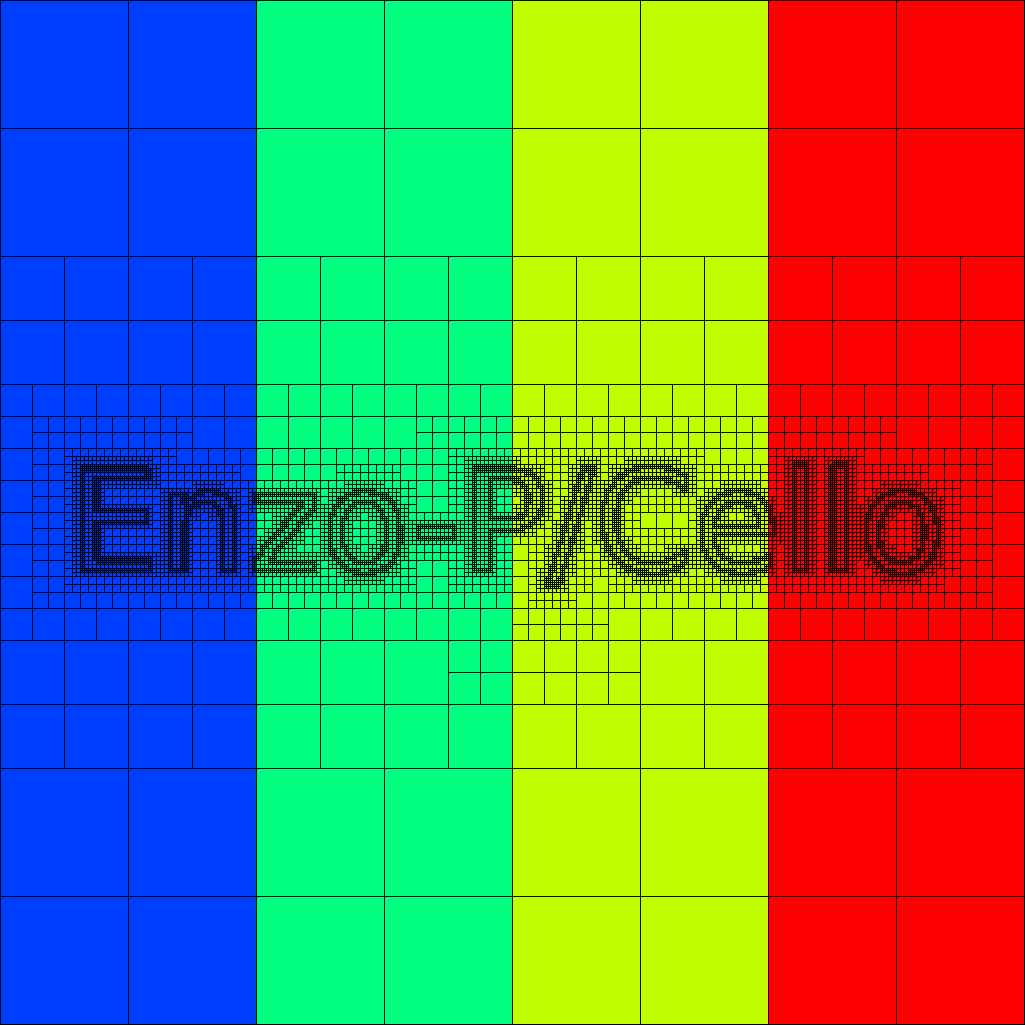
\includegraphics[width=1.3in]{Images/Balance/balance-mesh-00000.png}
\end{minipage}
\begin{minipage}{1.3in}
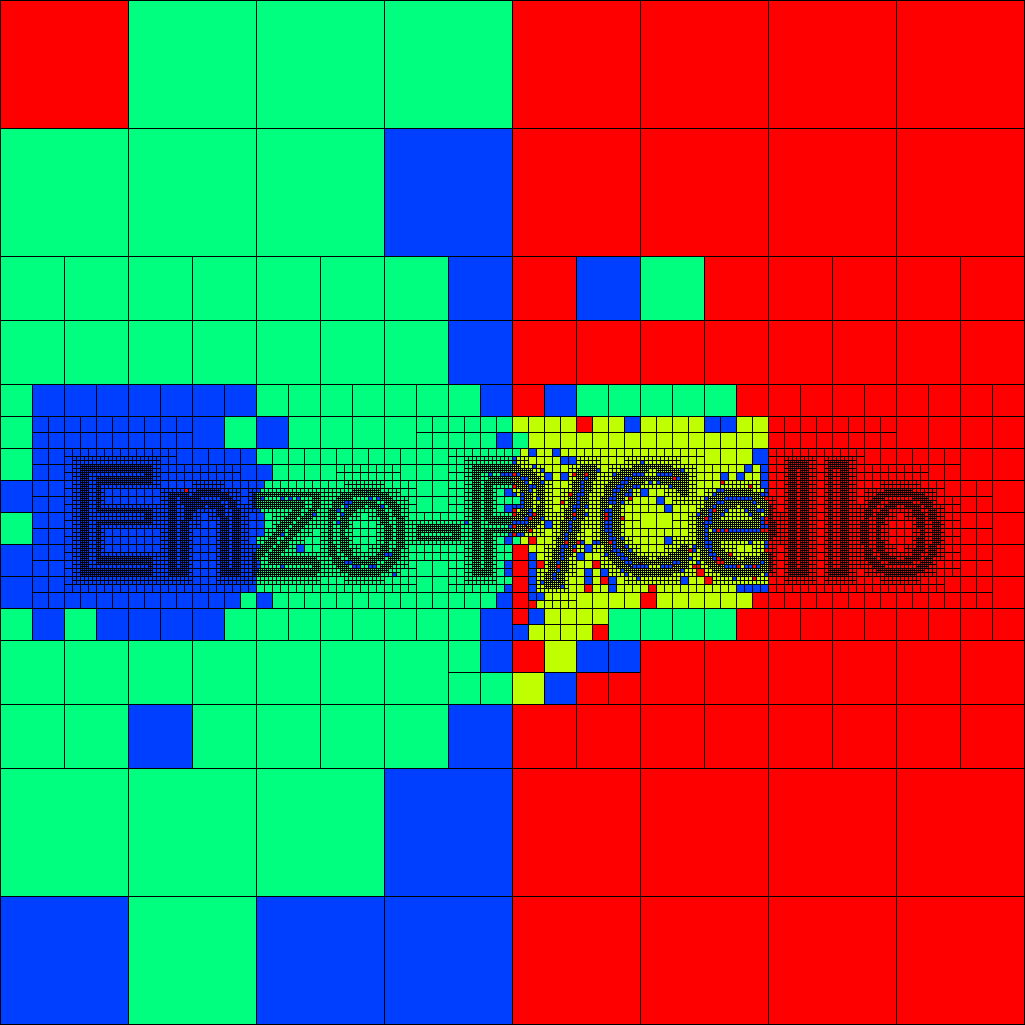
\includegraphics[width=1.3in]{Images/Balance/balance-mesh-00002.png}
\end{minipage}
\begin{minipage}{1.3in}
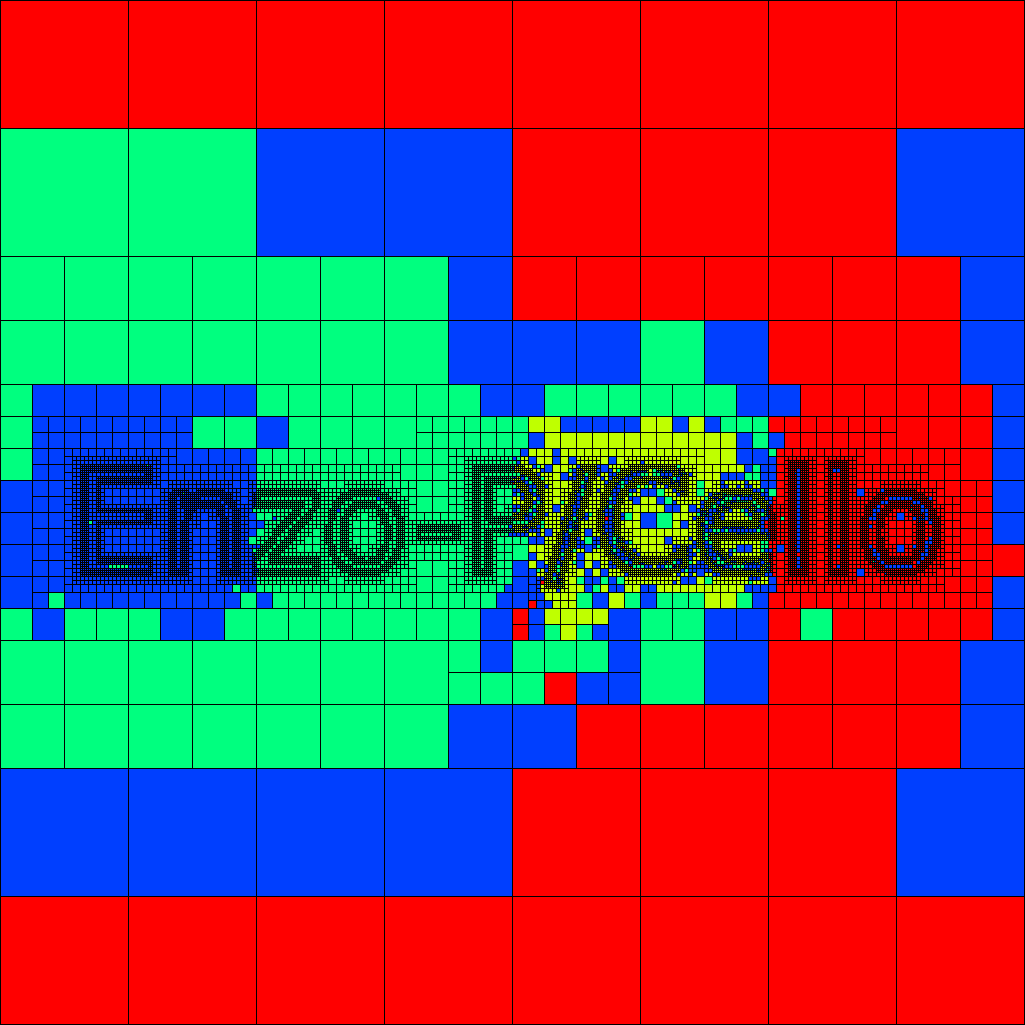
\includegraphics[width=1.3in]{Images/Balance/balance-mesh-00004.png}
\end{minipage}
\begin{minipage}{1.3in}
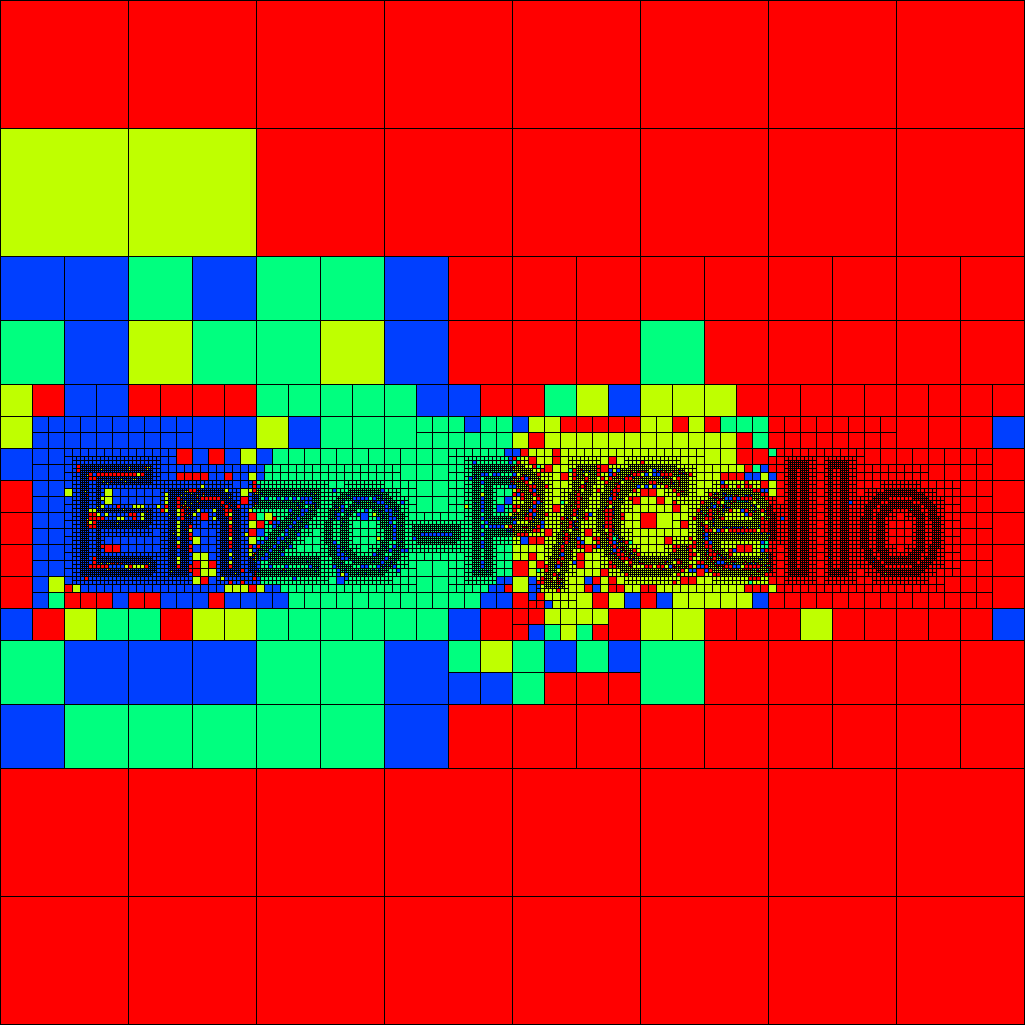
\includegraphics[width=1.3in]{Images/Balance/balance-mesh-00006.png}
\end{minipage}
\begin{minipage}{1.3in}
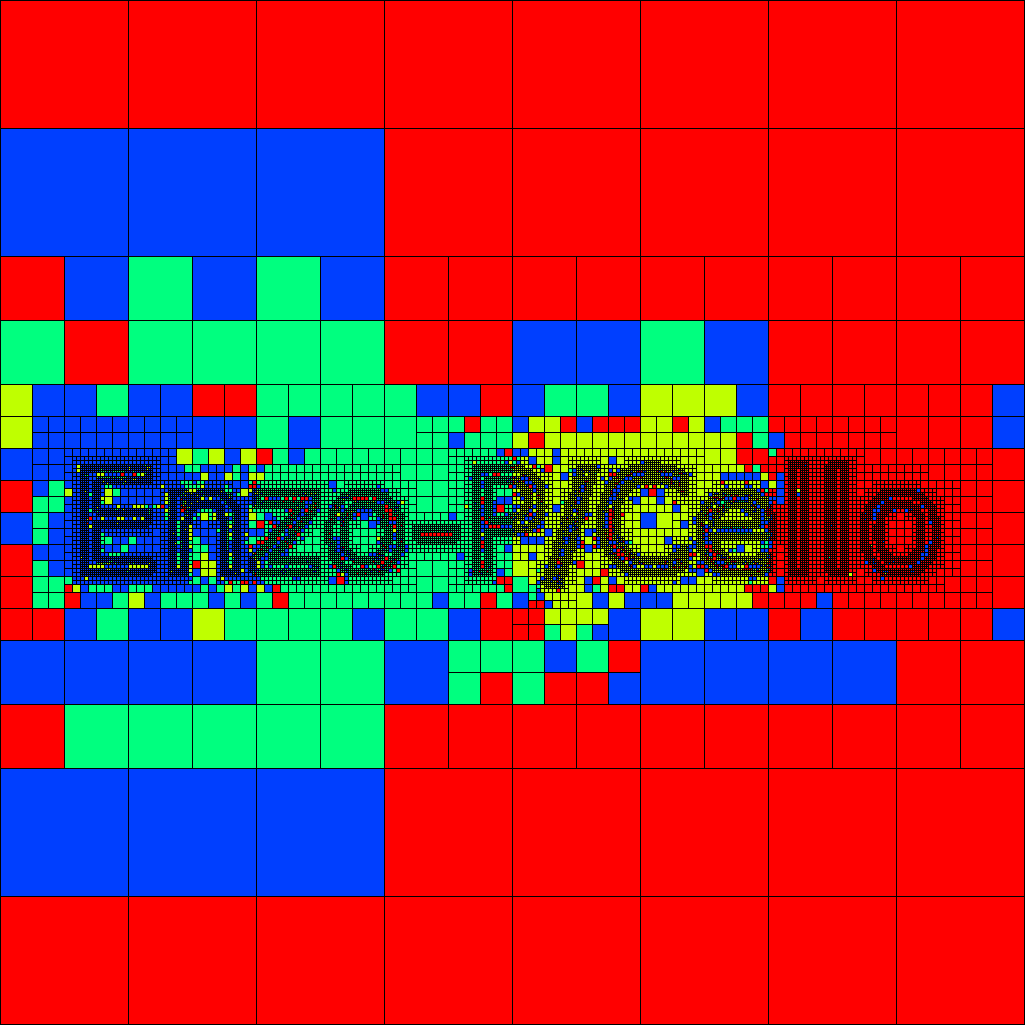
\includegraphics[width=1.3in]{Images/Balance/balance-mesh-00008.png}
\end{minipage}
\end{center}
\end{frame}
%----------------------------------------------------------------------



%     ComboCentLB : A special load balancer that can be used to combine any number of centralized load balancers mentioned above.

%     GreedyCommLB : Extends the greedy algorithm to take the communication graph into account.
%     GreedyLB : Uses a greedy algorithm that always assigns the heaviest object to the least loaded processor.
%     MetisLB : Uses METIS TM to partitioning object communication graph.
%     RandCentLB : Randomly assigns objects to processors;
%     RefineCommLB : Same idea as in RefineLB, but takes communication into account.
%     RefineLB : Moves objects away from the most overloaded processors to reach average, limits the number of objects migrated.
%     RefineSwapLB : Moves objects away from the most overloaded processors to reach average. In case it cannot migrate an object from an overloaded processor to an underloaded processor, it swaps objects to reduce the load on the overloaded processor. This strategy limits the number of objects migrated.
%     RefineTopoLB : Same idea as in RefineLB, but takes processor topology into account.
%     TopoCentLB : Extends the greedy algorithm to take processor topology into account.
 % How do run with dynamic load balancing?
%======================================================================
\NEWSEC
%======================================================================

\subsection{\ssTools}

\begin{frame}[fragile,label=ss-tools] 
\secframetitle{\ssTools}

% ch-perf.py
% ch-perf.sh
% ch-swf.sh
% diff-org.sh
% grep-org.sh
% log-org.sh
% ls-org.sh
% plot_mesh.py
\begin{description}
\pause
\item[\code{./build.sh}] \ \\ compile \enzop, compile and/or run regression tests
\pause
\item[\code{./tools/org-diff.sh}] \ \\ Create \bluecode{diff.org} \code{org-mode} file from \bluecode{hg diff}
\pause
\item[\code{./tools/org-log.sh}] \ \\ Create \bluecode{log.org} \code{org-mode} file from \bluecode{hg log}
\pause
\item[\code{./tools/plot\_mesh.py}] \ \\ Plot octree forest given block id's (e.g. \textit{B0:000\_1:001})
\pause
\item[\code{./tools/ch-swf.sh}] \ \\ Generate SWF (flash) file given a sequence of PNG files
\end{description}
\end{frame}

%----------------------------------------------------------------------

% \begin{frame}[fragile] 
% \secframetitle{\ssTools}
% \framesubtitle{\code{build.sh}}
% \end{frame}

%----------------------------------------------------------------------

% \begin{frame}[fragile] 
% \secframetitle{\ssTools}
% \framesubtitle{\code{org-diff.sh}}
% \end{frame}

%----------------------------------------------------------------------

% \begin{frame}[fragile] 
% \secframetitle{\ssTools}
% \framesubtitle{\code{org-log.sh}}
% \end{frame}

%----------------------------------------------------------------------

% \begin{frame}[fragile] 
% \secframetitle{\ssTools}
% \framesubtitle{\code{plot\_mesh.py}}
% \end{frame}

%----------------------------------------------------------------------

% \begin{frame}[fragile] 
% \secframetitle{\ssTools}
% \framesubtitle{\code{ch-swf.sh}}
% \end{frame}

%       example: 
%       bin/enzo-p input/adapt-L5-P1.in
%        (Ctrl-C after adapt-0.h5, or edit input to add Schedule { cycle = 0; } (or wait))
%           h5ls adapt-0.h5 | head
%          B0:000_0:100             Group
%          B0:000_0:101             Group
%          B0:000_0:110             Group
%          B0:000_0:111             Group
%          B0:000_1:000             Group
%          B0:000_1:001             Group
%          B0:001_0:100             Group
%          B0:001_0:101             Group
%          B0:001_0:110             Group
%          B0:001_0:111             Group
%       h5ls adapt-0.h5 | tools/plot_mesh.py
%          explain e.g. B0:001_0:110
%    parse_error.awk

%    ch-mem.py
%    ch-mem.sh
%    ch-perf.py
%    ch-perf.sh
%    diff-org.awk
%    parse_ls.sh
%    parse_warning.awk


 % What tools does Cello provide?
%======================================================================
\NEWSEC
%======================================================================

\subsection{\ssStartingSummary}

%----------------------------------------------------------------------

\begin{frame}[fragile,label=ss-starting-summary] 
\secframetitle{\ssStartingSummary}
\begin{itemize}
\item Enzo-P / Cello is easy (in principle) to download and install
\item Few dependencies
\begin{itemize}
\item \charm, HDF5, libpng, (csh,bc))
\end{itemize}
\item Not many platforms tested to date
\begin{itemize}
\item \redtext{Compiling issues are not unexpected!}
\item Your feedback is important!
\end{itemize}
\item Load-balancing requires command-line argument
\item Restarting requires checkpoint directory
\end{itemize}
\vfill
\centerline{$\qed$}
\end{frame}

 % What tools does Cello provide?

